\section{Technical Tools for the Development}
Before delving into the details of the development of the two histological models, which are the heart of this work, it should be convenient to dwell on every tool employed during the design phase.

All the work has been done in a pure \texttt{Python} environment, using several already established libraries and writing on my own missing code, for some specific applications. All the code produced during the development, the images, and the data produced have been collected in a devoted repository on GitHub \cite{repo}. I decided to code in \texttt{Python} given the thriving variety of available libraries geared toward scientific computation, image processing, data analysis, and last but not least for its ease of use (compared to other programming languages).

In this section, it will follow a description, in no particular order, of the less common tools I used during my work.

\subsection{Quaternions}
Quaternions are, in mathematics, a number system that expands in four dimensions the complex numbers. They have been described for the first time by the famous mathematician William Rowan Hamilton in 1843. This number system define three independent \textit{imaginary} units $\bm{i}$, $\bm{j}$, $\bm{k}$ as in (\ref{eq:quat_rules}), which allows the general representation of a quaternion $\bm{q}$ is (\ref{eq:quat}) and its inverse $\bm{q}^{-1}$ (\ref{eq:inv_quat}) where $a,b,c,d$ are real numbers:

\begin{align}
    \bm{i}^2 & = \bm{j}^2 = \bm{k}^2 = \bm{i}\bm{j}\bm{k} = -1, \label{eq:quat_rules}\\
    \bm{q} & = a + b\bm{i} + c\bm{j} + d\bm{k}, \label{eq:quat}\\
    \bm{q}^{-1 } = (a + b\bm{i} + c\bm{j} + d\bm{k})^{-1} & = \frac{1}{a^2 + b^2 + c^2 +d^2}\ (a - b\bm{i} - c\bm{j} - d\bm{k}). \label{eq:inv_quat}
\end{align}

Furthermore, the multiplication operation between quaternionn does not benefit from commutativity, hence the product between basis elements will behave as follows:

\begin{align}
    \bm{i} \cdot 1 = 1 \cdot \bm{i} = \bm{i}, & \qquad  \bm{j} \cdot 1 = 1 \cdot \bm{j} = \bm{j}, \qquad \bm{k} \cdot 1 = 1 \cdot \bm{k} = \bm{k} \label{eq:Ham_prod}\\
    & \bm{i} \cdot \bm{j}= \bm{k}, \qquad \bm{j} \cdot \bm{i}= -\bm{k} \nonumber \\
    & \bm{k} \cdot \bm{i}= \bm{j}, \qquad \bm{i} \cdot \bm{k}= -\bm{j} \nonumber \\
    & \bm{j} \cdot \bm{k}= \bm{i}, \qquad \bm{k} \cdot \bm{j}= -\bm{i}. \nonumber
\end{align}

This number system has plenty of peculiar properties and applications, but for the purpose of this project, quaternions are important for their ability to represent, in a very convenient way, rotations in three dimensions. In fact, the particular subset of quaternions with vanishing real part ($a=0$) has a useful, yet redundant, correspondence with the group of rotations in tridimensional space. Every 3D rotation of an object can be represented by a 3D vector $\vec u$: the vector's direction indicates the axis of rotation and the vector magnitude $|\vec u|$ express the angular extent of rotation. However, the matrix operation which expresses the rotation around an arbitrary vector $\vec u$ it is quite complex and does not scale easily for multiple rotations \cite{10.1007/BFb0031048}, which brings to very heavy and entangled computations.

Using quaternions for expressing rotations in space, instead, it is very convinient. Given the unit rotation vector $\vec u$ and the rotation angle $\theta$, the corresponding rotation quaternion $\bm{q}$ becomes (\ref{eq:rot_quat}):
\begin{align}
    \vec u & = (u_x, u_y, u_z) = u_x\bm{i} + u_y\bm{j} + u_z\bm{k}, \\
    \bm{q} & = e^{\frac{\theta}{2}(u_x\bm{i} + u_y\bm{j} + u_z\bm{k})} = \cos{\frac{\theta}{2}} + (u_x\bm{i} + u_y\bm{j} + u_z\bm{k})\sin{\frac{\theta}{2}}, \label{eq:rot_quat}\\
    \bm{q}^{-1} & = \cos{\frac{\theta}{2}} - (u_x\bm{i} + u_y\bm{j} + u_z\bm{k})\sin{\frac{\theta}{2}},
\end{align}
where in (\ref{eq:rot_quat}) we can clearly see a generalization of the Euler's formula for the exponential notation of complex numbers, which hold for quaternions. It can be shown that the application of the rotation represented by $\bm{q}$ on an arbitrary 3D vector $\vec v$ should be easily expressed as:
\begin{equation}
    \vec v\,' = \bm{q} \vec v \bm{q}^{-1},
\end{equation}
using the Hamilton product defined on quaternions (\ref{eq:Ham_prod}). This rule raises a very convinient and an extremily scalable way to compute consecutive rotations in space. Given two independent and consecutive rotations represented by the two quaternions $\bm{q}$ and $\bm{p}$ applyed on the vector $\vec v$ the resulting rotated vector $\vec v\,'$ is simply yielded as:
\begin{equation}
    \vec v\,' = \bm{p} ( \bm{q} \vec v \bm{q}^{-1} ) \bm{p}^{-1} = (\bm{p}\bm{q}) \vec v (\bm{q}\bm{p})^{-1},
\end{equation}
which essentially is the application of the rotation $\bm{r} = \bm{q}\bm{p}$ on the vector $\vec v$. This representation is completely coherent with the algebra of 3D rotations, which does not benefit from commutativity in turn.

Given this convenient property, quaternions are indeed widely used in all sorts of applications of digital 3D space design, as for simulations and for videogame design. The position of an object in the space in simulations is generally given by the application of several independent rotations, typically in the order of a tenth of rotations, which with quaternions is given easily by the product of simple objects. Every other alternative method would imply the use of matrix representation of rotations or other rotation systems as Euler's angles and would eventually make the computation prohibitive.

The use of quaternions in this work will be justified in section [??], while speaking of parametric L-systems in 3D space, used to build the backbone of the ramified structure of blood vessels in the reconstruction of a sample of pancreatic tissue.

I was able to find many useful \texttt{Python} libraries for computation with quaternions, but the one I appreciated the most for its interface and ease of use was the \texttt{pyquaternion}. With this library, it's almost immediate the definition of a quaternion by its correspondent rotation vector, and the multiplication between quaternions is very reliable.

\subsection{Parametric L-Systems} \label{ssec:Lsys}
Lindenmayer systems, or simply L-systems,  were conceived as a mathematical theory of plant development \cite{lindenmayer1968mathematical} in 1968 by Aristid Lindenmayer. Successively, a lot of geometrical interpretations of L-systems were proposed with the intention to make them a versatile instrument for modeling the morphology typical of plants and other organic structures. As a biologist, Lindenmayer studied different species of yeast and fungi and worked the growth patterns of various types of bacteria (e.g. as the \textit{cyanobacteria Anabaena catenula}). The main purpose for which L-systems were devised was to allow a formal description of the development of simple multicellular living organisms. Subsequently, the potentiality of these systems was expanded to describe higher-order plants and complex branching structures.

An L-system is in general defined by an \textit{axiom} sequence and some development \textit{rules}, which are recursively applied to the sequence and lead its development. The original proposed L-system was fairly simple and shows really well the idea underneath:
\begin{align}
    & axiom\ :\ A \nonumber \\
    & rules\ :\ (A \rightarrow AB),\quad(B \rightarrow A) \nonumber
\end{align}
where $A$ and $B$ could be any two different patterns in the morphology of an algae, or could be different bifurcations in a ramificated structure. The iterative application of the rules to the axiom sequence, let's say for 7 times, will produce the following sequence:
\begin{align}
    n = 0 &\ : A \nonumber \\
    n = 1 &\ : AB \nonumber \\
    n = 2 &\ : ABA \nonumber \\
    n = 3 &\ : ABAAB \nonumber \\
    n = 4 &\ : ABAABABA \nonumber \\
    n = 5 &\ : ABAABABAABAAB \nonumber \\
    n = 6 &\ : ABAABABAABAABABAABABA \nonumber \\
    n = 7 &\ : ABAABABAABAABABAABABAABAABABAABAAB\,. \nonumber
\end{align}

This kind of tool, as will be shown also in [??], is particularly suited for the creation of structures with fractal behavior, and it has been used in this work to create the backbone of the entangled bifurcation in blood vessels in the modelization of pancreatic tissue. In particular, there was the need for a fractal-like space-filling ramification as the one shown in Figures \ref{fig:bf_ls}. %and \ref{fig:full_ram}.

\begin{figure}
    \centering
    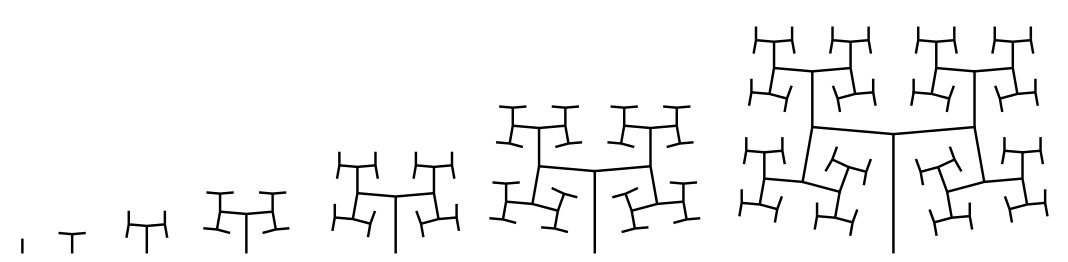
\includegraphics[width = 0.7\textwidth]{images/bf_ls}
    \caption{Growth pattern for the space-filling fract-like system, used to mimic the blood vassel bifurcations in sec [??]}
    \label{fig:bf_ls}
\end{figure}

%MAYBE THIS PICTURE IS REDUNDANT
% \begin{figure}
%     \centering
%     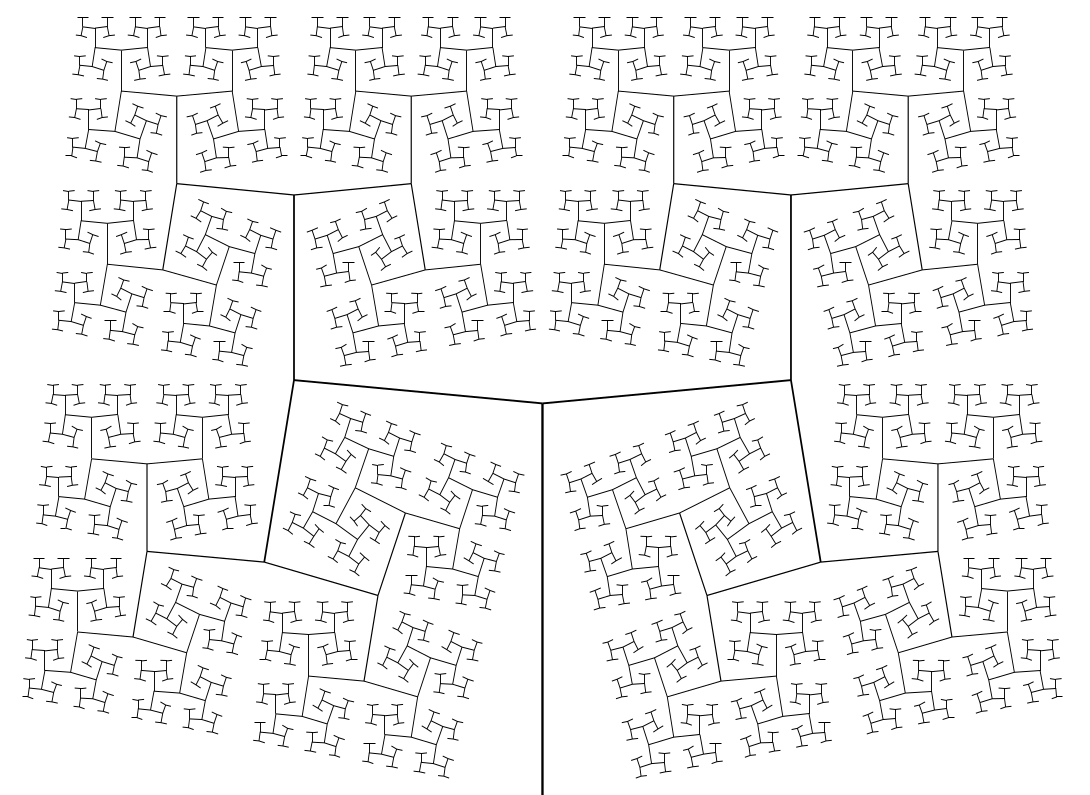
\includegraphics[width = 0.7\textwidth]{images/full_ram}
%     \caption{oijijo}
%     \label{fig:full_ram}
% \end{figure}

The system in Figure \ref{fig:bf_ls} represent the successive ramification of a structure which grows adding segments gradually shorter, by a ratio parameter $R$ and inclined of $\delta = \pm 85 \degree$ respect the previous branch. The axiom and the rules that produce this structure are the following:

\begin{align}
    & axiom\ :\ A \label{eq:bif_rules} \\
    & rule_1\ :\ A \rightarrow → F(1)[+A][-A] \nonumber \\
    & rule_2\ :\ F(s) \rightarrow F(s\cdot R) \nonumber
\end{align}
where $A$ represent the start of a new branch  and $F(s)$ represent a branch of lenght $s$. The presence of a rule which acts dfferently depending on the target object, is an further sophistication respect to the standard L-system. For this reason these systems are called parametric L-systems.

The use of standard L-systems turned out to be widespread, and there were a lot of different \texttt{Python} libraries at my disposal for coding. By the way, parametric L-systems were not just as popular, and I was not able to find a reliable library on which to build my work. I decided then to code a parametric branching system able to recreate the structure with rules (\ref{eq:bif_rules}) at any desired level of iteration. Creating the tool I needed on my own I was able to add all the optional features I would have needed during the development, like an adjustable degree of angular noise in the branch generation.

\subsection{Voronoi Tassellation} \label{ssec:vor_tass}
Voronoi diagrams, or Voronoi decompositions, are space-partitioning systems, which divides an $n$-dimensional Euclidian space into sub-regions depending on the proximity to a given set of objects. More precisely, given an $n$-dimensional space and $m$ starting point $p_1,\dots, p_m$ inside it, the whole space will be subdivided in $m$ adjacent regions. Every point of the space is assigned to the region correspondent to the nearest starting point. In Figure \ref{fig:vor_20} is shown a practical example of a Voronoi decomposition of a plane into 20 regions corresponding to the 20 starting points. Informal use of Voronoi diagrams can be traced back to Descartes in 1644, and many other mathematicians after him. But, Voronoi diagrams are named after Georgy Feodosievych Voronoy who defined and studied the general n-dimensional case in 1908 \cite{VoronoiNouvellesAD}.
\begin{figure}
    \centering
    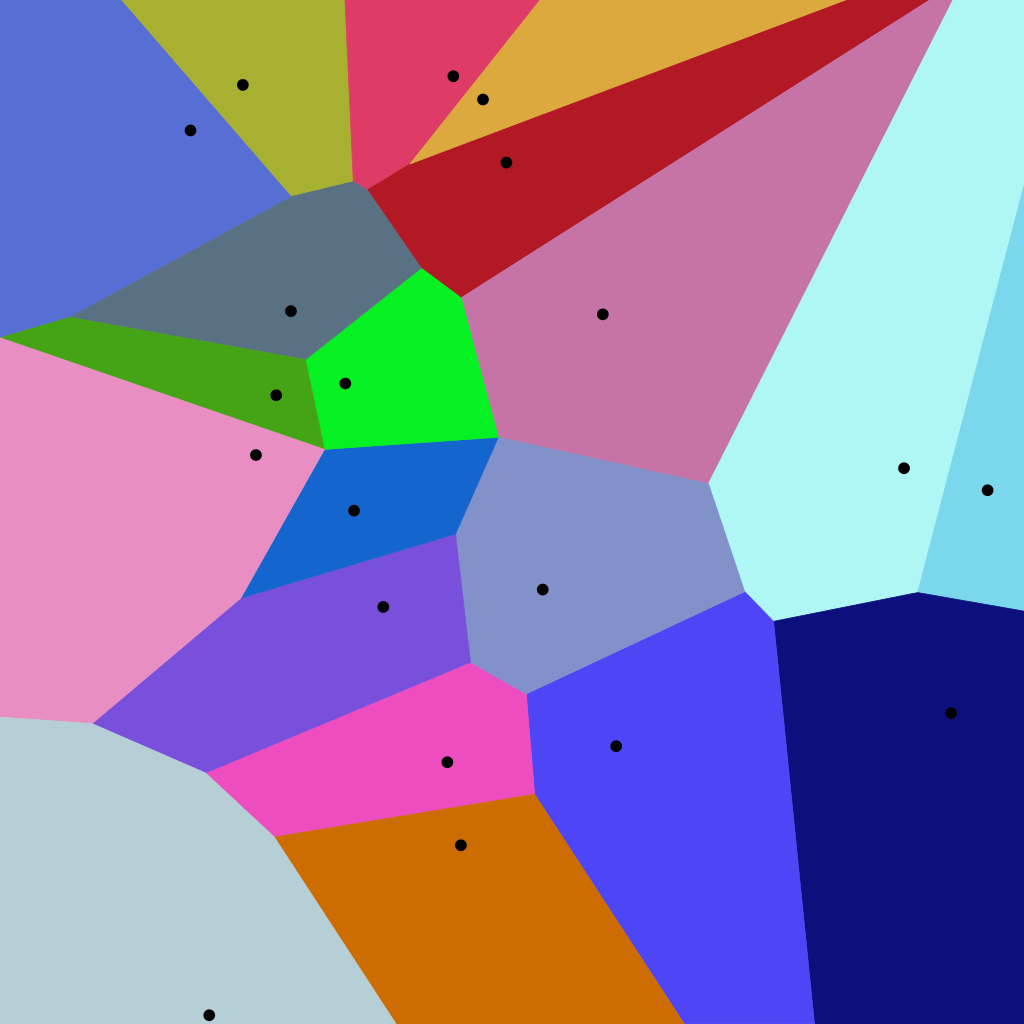
\includegraphics[width = 0.5\textwidth]{images/vor_20}
    \caption{Example of a Voronoi decomposition of a plane into 20 regions corresponding to 20 starting points}
    \label{fig:vor_20}
\end{figure}

More precisely, let $X$ be a metric space and $d$ the distance defined on it. Let $K$ be the set of indices and let $(P_k)_{k\in K}$ be the tuple of sites in the space $X$. The $k^{th}$ Voronoi cell $R_k$, associated with the site $P_k$ is the set of all the points in $X$ whose distance to $P_k$ is smaller than the distance to any other site $P_j$, with $j\neq k$, or in other words:
\begin{equation}
    R_k = \{x \in X\;|\;d(x,P_k) \le d(x,P_j)\; \forall j \in K, \;j\neq k \}, \label{eq:formal_Vor_def}
\end{equation}
depending on the notion of distance defined on the space $X$ the final redistribution in subregions will look very differently.

In addittion to the choice of the distance function, another foundamental factor is the dstribution of sites in the space to be divided. If the points are chosen equally and omogenously distributed the final distribution will appear as a simple regular lattice, while a complete random distribution of points in the space will provide a decomposition in cells with very different shapes and volumes, as shown in Figure \ref{fig:diff_pt}. Interesting results concerning points from a semi-random distribution will be shown in section [??], which lead to a decomposition with a good richness in shapes but with the desired homogeneity in volumes.
\begin{figure}
    \centering
    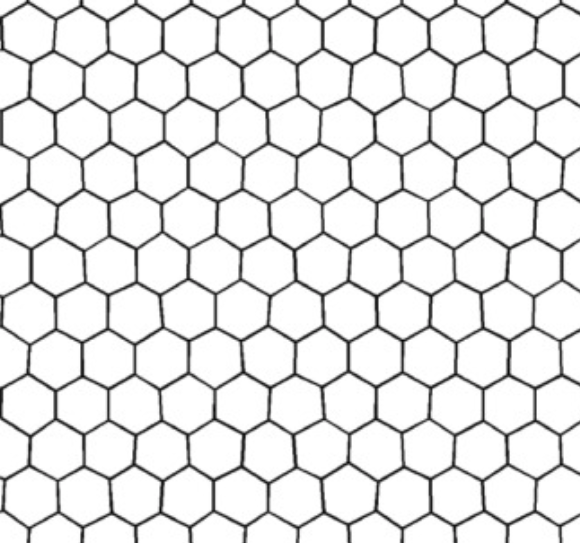
\includegraphics[width = 0.4\textwidth]{images/reg_pt}
    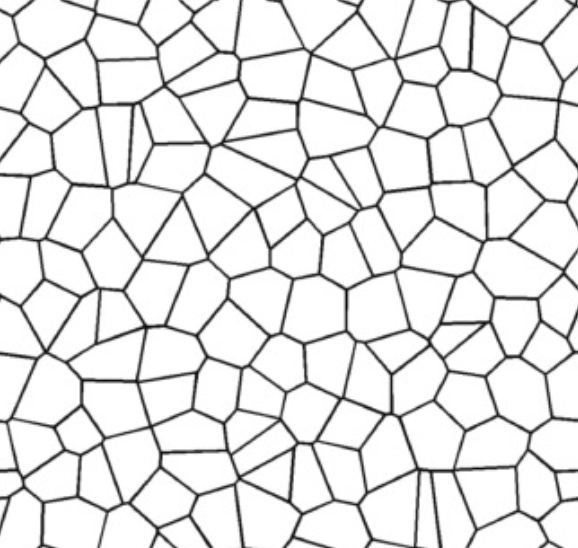
\includegraphics[width = 0.4\textwidth]{images/ran_pt}
    \caption{On the right an example of 2D Voronoi decomposition resulting from a omogenously distribuited points in the plane. On the left the resulting decomposition obtained from randomly distribuited points in the plane, from \cite{ALSAYEDNOOR201644}.}
    \label{fig:diff_pt}
\end{figure}

The Voronoi Decomposition has been of great interest in this project for the division of a 3D space in subregions, to recreate the spatial distribution of cells in a sample of human tissue, as will be shown in section [??]. The formal definition of Voronoi regions \ref{eq:formal_Vor_def} ensure the convexity of each decomposition's tassel, which in three-dimensional space would be adjacent convex polyhedrons. Every tassel of the decomposition will be represented by a bounded 3-dimensional convex hull \footnote{See section \ref{ssec:pol_sec} for further details.}, with  except for those most external cells which are unbounded and requires special attention while using.

The most widespread tool for the computation of Voronoi decompositions in \texttt{Python} is contained in the \texttt{spatial} submodule of the famous library \texttt{SciPy}, which is a staple tool for an incredible variety of scientific algorithms. The \texttt{Voronoi} object from \texttt{Scipy} library offers a very efficient algorithm for space-partitioning, and it has been one of the pillars for the modelization of tissues.

\subsection{Saltelli Algorithm - Randon Number Generation}
\begin{figure}
    \centering
    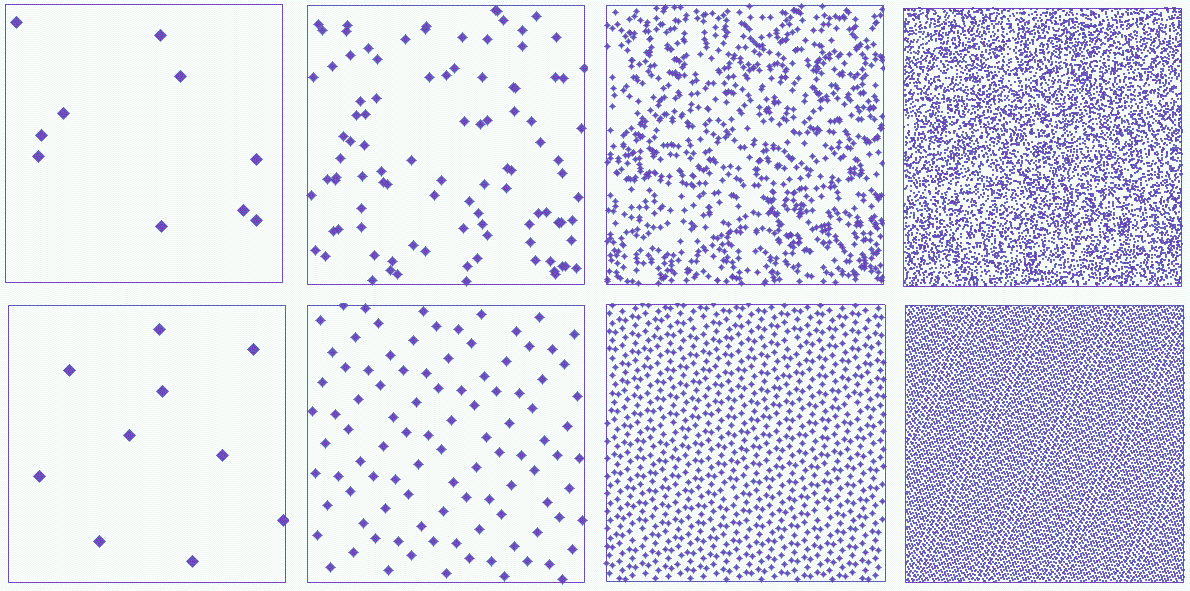
\includegraphics[width = 0.7\textwidth]{images/Subrandom_2D}
    \caption{Coverage of the unit square with an additive quasirandom numbers sequence as in \ref{eq:ad_rec} (UP) and  for uniformly sampled random numbers (BOTTOM). From top to bottom: 10, 100, 1000, 10000 points.}
    \label{fig:Subrandom_2D}
\end{figure}
As mentioned in section \ref{ssec:vor_tass}, in this project there was the need of quasi-random number generation for the production of Voronoi tassellations. Quasi-random sequences (or low-discrepancy sequences) are patterns of numbers which emulate the behaviour of uniform random distributions, but have a more homogeneous and quick coverage of the sampling domain, which provide an important advantege in applications as in quasi-Monte Carlo integration techniques, as shown in Figure \ref{fig:Subrandom_2D}. In computer science there is not any possibility of recreating \textit{true} random sequences, hence any stocasticity is completely deterministic in its essence even if produced by very chaotic processes \footnote{A chaotic process is a deterministic process which has an extremily sensible dependence on its starting conditions. This property mimics very effectively the behaviour of true random processes, which are intrinsically forbidden in computer science.}. Indeed, every algorithm for random number generation is completely repeatable given its starting status. Quasi-random sequences, are completely deterministic too, but implements more \textit{predictable} algorithm.

A first good example to understand the concept of quasi-random generation could be an additive reccurrence, as the following:
\begin{equation}
    s_{n+1} = ( s_n + \alpha ) \bmod 1,
    \label{eq:ad_rec}
\end{equation}
which for every seed element $s_0$ and real parameter $\alpha$ produced completely different sequences.

\hl{[THE FOLLOWING PARAGRAPH SOUNDS TOO HEAVY AND TECHNICAL]}

In the bottom line of Figure \ref{fig:Subrandom_2D} is clearly visible the good and homogeneous coverage of the sampling domain, altough it strongly visible a regular pattern between points, which does not convey an \textit{organic} sensation at all. However, increasing the complexity of our very simple starting model \ref{eq:ad_rec} it is possible to overcome this \textit{artificial} appereance of sampled points and to produce very good samples.

A notorious algorithm for quasi-random number generation is the Sobol sequence, introduced by the russian mathematician Ilya M. Sobol in 1967 \cite{SOBOL2001271}. In its work, Sobol wanted to construct a sequence $x_n$ of points in the $s$-dimensional unitary hybercube $I^s = [0,1]^s$ such as for any integrable function $f$:
\begin{equation}
    \lim_{n\to\infty} \frac{1}{n} \sum_{i=1}^{n} f(x_i) = \int_{I_s} f.
\end{equation}
Sobol wanted to minimize the \textit{holes} in the sampled domain (which it could be shown to be a property that helps the convergence of the sequence) and minimize as well the \textit{holes} in every lower-dimension projection of the sampled points. The particularly good distributions that fullfill those requirments are known as $(t,m,s)$-nets and $(t,s)$-sequences in base $b$. To better understand them we need first to define the concept of $s$-interval in base $b$, which is a subset of $I_s$ such as:
\begin{equation}
    E_s^b = \prod_{j=1}^{s} \Bigg[ \frac{a_j}{b^{\,d_j}}, \frac{a_j + 1}{b^{\,d_j}}\Bigg),
\end{equation}
where $a_j$ and $d_j$ are non-negative integers, and $a_j < b^{d_j}$ for all j in \{1, ...,s\}.

Let be $t$ and $m$ two integers such as $0 \leq t \leq m$. A $(t,m,s)$-net in base $b$ is defined as a sequence $x_n$ of $b^m$ points of $I_s$ such that:
\begin{equation}
    \mathbf{Card} \ \mathbf{P} \cap \{x_1, \dots, x_n \} = b^t
\end{equation}
for all the elementary  interval $\mathbf{P}$ in base $b$ of hypervolume $\lambda(\mathbf{P}) =  b^{t-m}$.

Given a non-negative integer $t$, a $(t,s)$-sequence in base $b$ is an infinite sequence of points $x_n$ such that for all integers $k \geq 0$, $m \geq t$ the sequence $ \{ x_{kb^m}, \dots, x_{(k+1)b^m-1} \}$ is a $(t,m,s)$-net in base $b$.

Sobol in his article described in particular $(t,m,s)$-net and $(t,s)$-sequence in base 2. A more torough description of all the formal properties of those particular sequences could be find in \cite{SOBOL1976236}.

In order to perform the actual sampling during the modelization, it has been used the \texttt{saltelli} module from the \texttt{SALib} library, which performs a sampling in an $s$-dimensional space following the Saltelli algorithm, which is a specific improved version of the Sobol algorithms oriented toward the parameter sensitivity analysis \cite{SALTELLI2002280}, \cite{SALTELLI2010259}.

\subsection{Planar Section of a Polyhedron} \label{ssec:pol_sec}
As will be shown in section [??] a foundamental step for the functioning of the modelization is the planar section of a three dimensional polyhedron. It tourned out that there is no general rule to perform a planar section of a convex polyhedron with an arbitrary number of faces, respect to an arbitrary sectioning plane. Hence, I devised an algorithm to handle this task. In the general case the result of the sectioning process of a polyhedron is a polygonal surface in the case of full intersection. Otherwise it could be an empty set of points or a segment in case of particular tangency, but those two cases are not of interest for the model.

Given a convex polyhedron with $n$ vertices and the a sectioning plane $p$, let $V$ be the set of all the vertices and $f_p(\vec x)$ the equation defining the plane. The algorithm is defined by the following steps:
\begin{enumerate}
    \item Divide the $V$ in two subsets: $A$ made of those vertices which lie above and $B$, made of those which lie below the sectioning plane. Like in \ref{eq:ab_bel}:
    \begin{align}
        A = \{ v \in V \ |\ f_p(v)\geq 0\} \label{eq:ab_bel} \\
        B = \{ v \in V \ |\ f_p(v)\leq 0\} \nonumber
    \end{align}
    If any of the two subsets tourns out to be empty the plane $p$ does not intersect the polyhedron, and the section is empty. $A$ and $B$ are represented in different colors in Figure \ref{fig:pol_sec}.

    \item Detect, and \textit{draw}, any possible line that crosses two points respectively from $A$ and $B$. If $n_A$ and $n_B$ are the number of points above and below the plane then there will be $n_A \times n_B$ possible lines. In Figure \ref{fig:pol_sec} all the lines between the two classes of point are drawn in white.

    \item Detect all the points $P$ from the intersection between the $n_A \times n_B$ lines from the previous step and the sectioning plane $p$. All these points will lie on the same plane, within the boundaries of the polygonal section.

    \item The final polygon, is then yielded by computing the convex hull of the points in $P$. The convexity of the starting polyhedron in fact ensure the convexity of any section of the solid.
\end{enumerate}




\begin{figure}
    \centering
    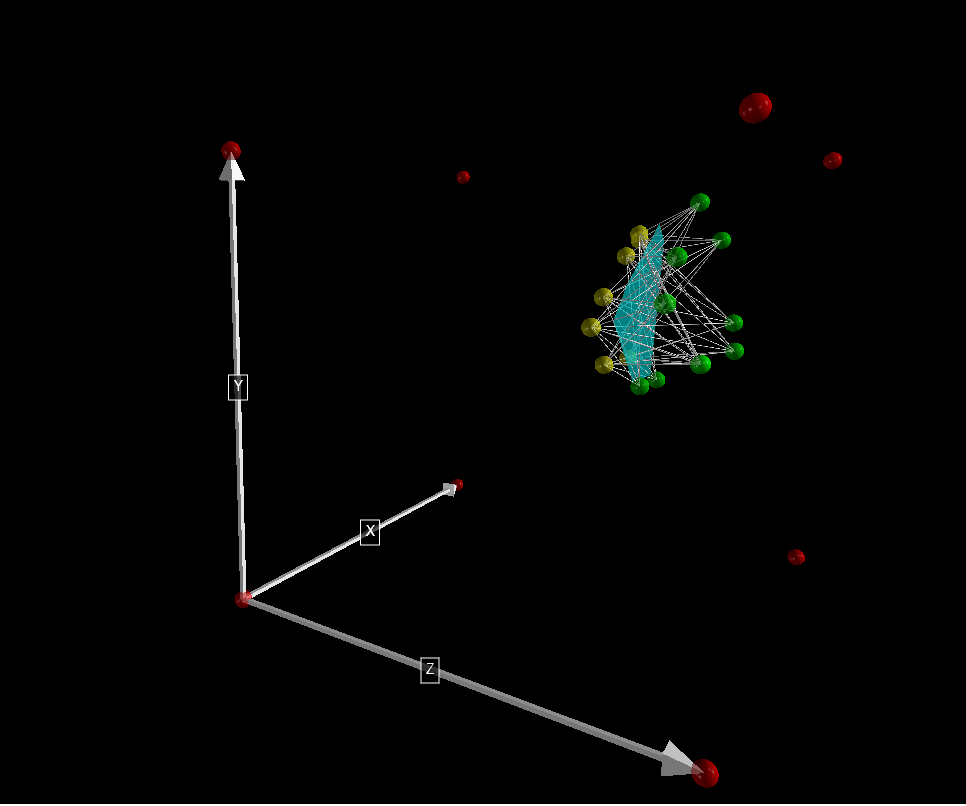
\includegraphics[width = 0.7\textwidth]{images/pol_sec}
    \caption{....}
    \label{fig:pol_sec}
\end{figure}



\subsection{VPython - 3D Visualization}

\subsection{SnakeMake}

\subsection{Perlin Noise}

\subsection{Style-Transfer Neural Network}\label{ssec:sttrNN}
